% Options for packages loaded elsewhere
\PassOptionsToPackage{unicode}{hyperref}
\PassOptionsToPackage{hyphens}{url}
%
\documentclass[
]{article}
\title{Impact of cropping system diversification on vegetative and reproductive characteristics of waterhemp (\emph{Amaranthus tuberculatus})}
\author{}
\date{\vspace{-2.5em}}

\usepackage{amsmath,amssymb}
\usepackage{lmodern}
\usepackage{iftex}
\ifPDFTeX
  \usepackage[T1]{fontenc}
  \usepackage[utf8]{inputenc}
  \usepackage{textcomp} % provide euro and other symbols
\else % if luatex or xetex
  \usepackage{unicode-math}
  \defaultfontfeatures{Scale=MatchLowercase}
  \defaultfontfeatures[\rmfamily]{Ligatures=TeX,Scale=1}
\fi
% Use upquote if available, for straight quotes in verbatim environments
\IfFileExists{upquote.sty}{\usepackage{upquote}}{}
\IfFileExists{microtype.sty}{% use microtype if available
  \usepackage[]{microtype}
  \UseMicrotypeSet[protrusion]{basicmath} % disable protrusion for tt fonts
}{}
\makeatletter
\@ifundefined{KOMAClassName}{% if non-KOMA class
  \IfFileExists{parskip.sty}{%
    \usepackage{parskip}
  }{% else
    \setlength{\parindent}{0pt}
    \setlength{\parskip}{6pt plus 2pt minus 1pt}}
}{% if KOMA class
  \KOMAoptions{parskip=half}}
\makeatother
\usepackage{xcolor}
\IfFileExists{xurl.sty}{\usepackage{xurl}}{} % add URL line breaks if available
\IfFileExists{bookmark.sty}{\usepackage{bookmark}}{\usepackage{hyperref}}
\hypersetup{
  pdftitle={Impact of cropping system diversification on vegetative and reproductive characteristics of waterhemp (Amaranthus tuberculatus)},
  hidelinks,
  pdfcreator={LaTeX via pandoc}}
\urlstyle{same} % disable monospaced font for URLs
\usepackage[margin=1in]{geometry}
\usepackage{longtable,booktabs,array}
\usepackage{calc} % for calculating minipage widths
% Correct order of tables after \paragraph or \subparagraph
\usepackage{etoolbox}
\makeatletter
\patchcmd\longtable{\par}{\if@noskipsec\mbox{}\fi\par}{}{}
\makeatother
% Allow footnotes in longtable head/foot
\IfFileExists{footnotehyper.sty}{\usepackage{footnotehyper}}{\usepackage{footnote}}
\makesavenoteenv{longtable}
\usepackage{graphicx}
\makeatletter
\def\maxwidth{\ifdim\Gin@nat@width>\linewidth\linewidth\else\Gin@nat@width\fi}
\def\maxheight{\ifdim\Gin@nat@height>\textheight\textheight\else\Gin@nat@height\fi}
\makeatother
% Scale images if necessary, so that they will not overflow the page
% margins by default, and it is still possible to overwrite the defaults
% using explicit options in \includegraphics[width, height, ...]{}
\setkeys{Gin}{width=\maxwidth,height=\maxheight,keepaspectratio}
% Set default figure placement to htbp
\makeatletter
\def\fps@figure{htbp}
\makeatother
\setlength{\emergencystretch}{3em} % prevent overfull lines
\providecommand{\tightlist}{%
  \setlength{\itemsep}{0pt}\setlength{\parskip}{0pt}}
\setcounter{secnumdepth}{-\maxdimen} % remove section numbering
\usepackage{lineno}
\linenumbers
\usepackage{float}
\usepackage{booktabs}
\usepackage{longtable}
\usepackage{array}
\usepackage{multirow}
\usepackage{wrapfig}
\usepackage{colortbl}
\usepackage{pdflscape}
\usepackage{tabu}
\usepackage{threeparttable}
\usepackage{threeparttablex}
\usepackage[normalem]{ulem}
\usepackage{makecell}
\usepackage{xcolor}
\ifLuaTeX
  \usepackage{selnolig}  % disable illegal ligatures
\fi
\usepackage[round]{natbib}
\bibliographystyle{plainnat}

\begin{document}
\maketitle

\hypertarget{appendix}{%
\section*{Appendix}\label{appendix}}
\addcontentsline{toc}{section}{Appendix}

\hypertarget{appendix-a}{%
\subsection{Appendix A:}\label{appendix-a}}

\emph{Seed cleaning and counting procedure}

The following protocol was used to separate seeds from stems and to clean seeds.

Step 1 - A whole sample was run through a brushing machine (LA-H, Westrup, Slageise, Denmark) to break the fruits from the stem. Large samples were chopped before running through the machine.

Step 2 - Chaff-covered seeds were run through a stack of two sieves (US Standard Sieve Series), one that was 710 micron on top and one that was 297 micron at the bottom in a shaker (Dayton, Seedburo Equipment Company). The sieve stack was securely closed with a top and a bottom lid. The 297-micron sieve was used to separate small stems, while the 710-micron sieve separated the dust from the seeds. Seeds at this step were still chaffy and partially enclosed in the fruits. Seeds that were still enclosed at this step did not pass the top sieve and were rubbed with rubber bands (Step 4). Small pieces of stems and dust were discarded. The material in between the two sieves was retained.

Step 3 - The material between the two sieves from step 2 was run through a custom-made dual-slope separator (Iowa State University Seed Laboratory) to separate clean seeds and chaffed seeds.

Step 4 - The pericarps from step 3 were rubbed in between rubber bands to remove capsules.

Step 5 - Seeds from steps 3 and 4 were run separately through a blower (CB-1, Agriculex Inc, Guelph, Canada) to remove the remaining capsules. The blower was started at the lowest wind speed and adjusted throughout the blowing process so that as much of the chaff and foreign materials were removed as possible while seeds were retained.

Step 6 - Steps 3 to 5 were repeated depending on the cleanliness of the material.

Step 7 - Cleaned seeds were enumerated with either an Old Mill Counter (850-3, International Marketing and Design Corp) or a Ball Coleman optical counter (Gen3, Ball Horticultural Company, Illinois, USA). The Ball Coleman optical counter was with a precision of 0.16\% difference between samples several times per sample. With the Old Mill Counter, seeds were counted once. With the Old Mill Counter or by hand, each sample was counted once. With the Ball Coleman optical counter, each sample was counted several times and three counts that were the least different from one another were averaged and used as the sample's seed count.

\emph{Seed sample preparation and machine calibration}

Seeds to be counted were threshed by hand or machine, depending on plant size, and then cleaned of chaff.
Samples of hundreds of seeds were counted by hand, larger samples with either an Old Mill Counter or a Ball Coleman optical Counter. Before counting, each sample bag was weighed, i.e., bag, tag, and plant material, then the bag and tag.
Plant weight was obtained by subtracting the bag and tag weight from the sample bag weight.
Seeds must be fairly clean in order to be counted with machines.
Obtaining clean seed samples without chaff and foreign materials was extremely time-consuming, so we trained an optical counter to eliminate particles whose sizes were noticeably different from the mean seed size of roughly 1 mm diameter \citep{bellTimeRequirementPollination2010}.
The Ball Coleman optical counter was calibrated to count waterhemp seeds by running a ``known sample'' of 1200 seeds (a sample that was counted by hand) to establish a learning function to eliminate particles that were very much smaller and larger than the mean seed size from the final count.
The ``known sample'' was run through the optical counter at 2300 seeds/second, uncalibrated, to obtain a distribution of all the counted particles.
The counting rate of 2300 seeds/second was automated by the counter after running a small batch of seeds in such a way that a steady, single-file seed flow was maintained during the counting process.
Two tails of the distribution of particle sizes, i.e., too large and too small, were trimmed in such a way that the new counts were closest to the hand-counted number.
In our case, any counted particles whose surface area was larger than 0.1963 mm\(^2\) were removed from the total count in the learning function.
Once the learning function was established, seeds were counted with reference to the saved settings.
The known sample was recounted with the calibrated counter to confirm the result.


\hypertarget{appendix-b-2019-sex-ratio-imputation}{%
\subsection*{Appendix B: 2019 sex ratio imputation}\label{appendix-b-2019-sex-ratio-imputation}}
\addcontentsline{toc}{subsection}{Appendix B: 2019 sex ratio imputation}

\hypertarget{data-set-and-imputation-procedure-overview}{%
\subsubsection*{Data set and imputation procedure overview}\label{data-set-and-imputation-procedure-overview}}
\addcontentsline{toc}{subsubsection}{Data set and imputation procedure overview}

The experiment design was randomized complete block design with four blocks, nine levels of main plot (Crop ID) and two levels of split-plot (Corn weed management) effects. There were 72 experimental units (eu), 8 observational units (quadrats) per eu. Within each quadrat, six cohorts of plants were sexed. By the time that the plants were sexed, a few plants' sexes were not observable, and thus, they were marked as Unknown in the data set. This caused Total \textgreater{} Male + Female in some eu's.

Complete case analysis, in which missing observations are removed from the data set, is acceptable when less than 5\% of the data is missing at random because removing the incomplete cases does not significantly change the outcome \citep{azurMultipleImputationChained2011}. The 2019 sex ratio is imputed because 22\% of the data (755 \texttt{NA}s out of 3456 entries (6 cohorts/quadrat x 8 quadrats/eu x 72 eu)) was missing at random (MAR). We considered our data MAR even though the number of missing values were higher in soybean plots than in the other three crops because 1) the quadrats were placed randomly in the field before weed emergence, 2) waterhemp and other weed seedlings were present in the quadrats at the beginning of the season, and 3) waterhemp and other weed species were found in soybean plots by the time we sexed the waterhemp plants, but not in the eight fixed quadrats.

The MICE imputation method assumes that after controlling for all the observations in the original data set, all the missingness occurs at random \citep{vanbuurenMiceMultivariateImputation2011}. A good imputation model is numerically recognized by low fraction of information missing due to nonresponse (\texttt{fmi}), small proportion of total variance that is attributable to the missing data (\(\lambda\)) values; and visually recognized by the similarity in kernel density estimates and data points distribution between the observed and imputed data sets \citep{vanbuurenMiceMultivariateImputation2011}. The number of imputations (m) should be chosen such that the loss of efficiency, \(le = \frac{fmi}{m} \leq 0.05\) \citep{whiteMultipleImputationUsing2011}. To give the imputation model more information, the data was imputed using 3456 data points. The analysis model on the imputed data sets was run using 72 data points. 

The recommended specifications of the imputation model for this data set are: 1) uses at least 24 imputations (24 was selected because it is divisible by 4 cores in the computer processor), 2) includes all the covariates (Number of emerged seedlings, Male, Female, and Total) and predictors in the analysis model, and 3) uses an overdispersed Poisson regression model \citetext{\citealp{azurMultipleImputationChained2011}; \citealp{whiteMultipleImputationUsing2011}; \citealp[and][]{nguyenModelCheckingMultiple2017}}. While the first two specifications were met, overdispersed Poisson regression model could not be specified. The extensions for count data mentioned in Chapter 7 \citep{vanbuurenFlexibleImputationMissing2018} do not fit this data set well. Both \texttt{micemd}'s \texttt{mice.impute.2l.glm.pois} and \texttt{mice.impute.2l.2stage.pois} functions impute the numbers of Male, Female, and Total separately \citep{audigierMicemdMultipleImputation2021}. The predictive mean matching (\texttt{pmm}) method in the \texttt{mice} package can handle counts \citep{vanbuurenMiceMultivariateImputation2011} and is the optimal solution for this data set at this writing (Figure \ref{fig:kernel-xy-imp1-all-diag}).

\hypertarget{diagnosis-of-the-imputation-model-with-m-24}{%
\subsubsection*{Diagnosis of the imputation model with m = 24}\label{diagnosis-of-the-imputation-model-with-m-24}}
\addcontentsline{toc}{subsubsection}{Diagnosis of the imputation model with m = 24}

The imputation code with predicted mean matching (\texttt{pmm}) method is provided in \citep{nguyenDataImpactCropping2022}. Each round of imputation is distinguished by the number of imputations (m). The loss of efficiency (le) are all below the recommended value of 0.05 \citep{whiteMultipleImputationUsing2011} for the analysis model terms using the imputed data sets, under three m values and the imputation performance improved as m increased (Table \ref{tab:pool-diag}). m was capped at 2400 imputations for this manuscript because of limited computational power. The diagnosis of data imputation is demonstrated here with m = 24 for ease of view. The distribution of the imputed data sets match that of the observation (Figure \ref{fig:kernel-xy-imp1-all-diag}) so the outputs (imputed data sets) were used for further regression analyses that involved sex ratio.

\hypertarget{diagnosis-of-the-analysis-model-with-m-24}{%
\subsubsection*{Diagnosis of the analysis model with m = 24}\label{diagnosis-of-the-analysis-model-with-m-24}}
\addcontentsline{toc}{subsubsection}{Diagnosis of the analysis model with m = 24}

The similarity in the magnitude of reduction of deviance and dispersion values suggests comparable, small impacts of population aboveground mass and population stand density covariates on the improvement of the goodness of fit for comparing sex ratio using 2019 imputed data \citep{nguyenDataImpactCropping2022}. In addition, using either of them as a covariate in the analysis models resulted in nonestimable corn weed management effects on sex ratios in some treatments, so 2019 sex ratios were averaged over corn weed management regimes and compared without any covariates for simplicity. 

\begin{figure}[H]
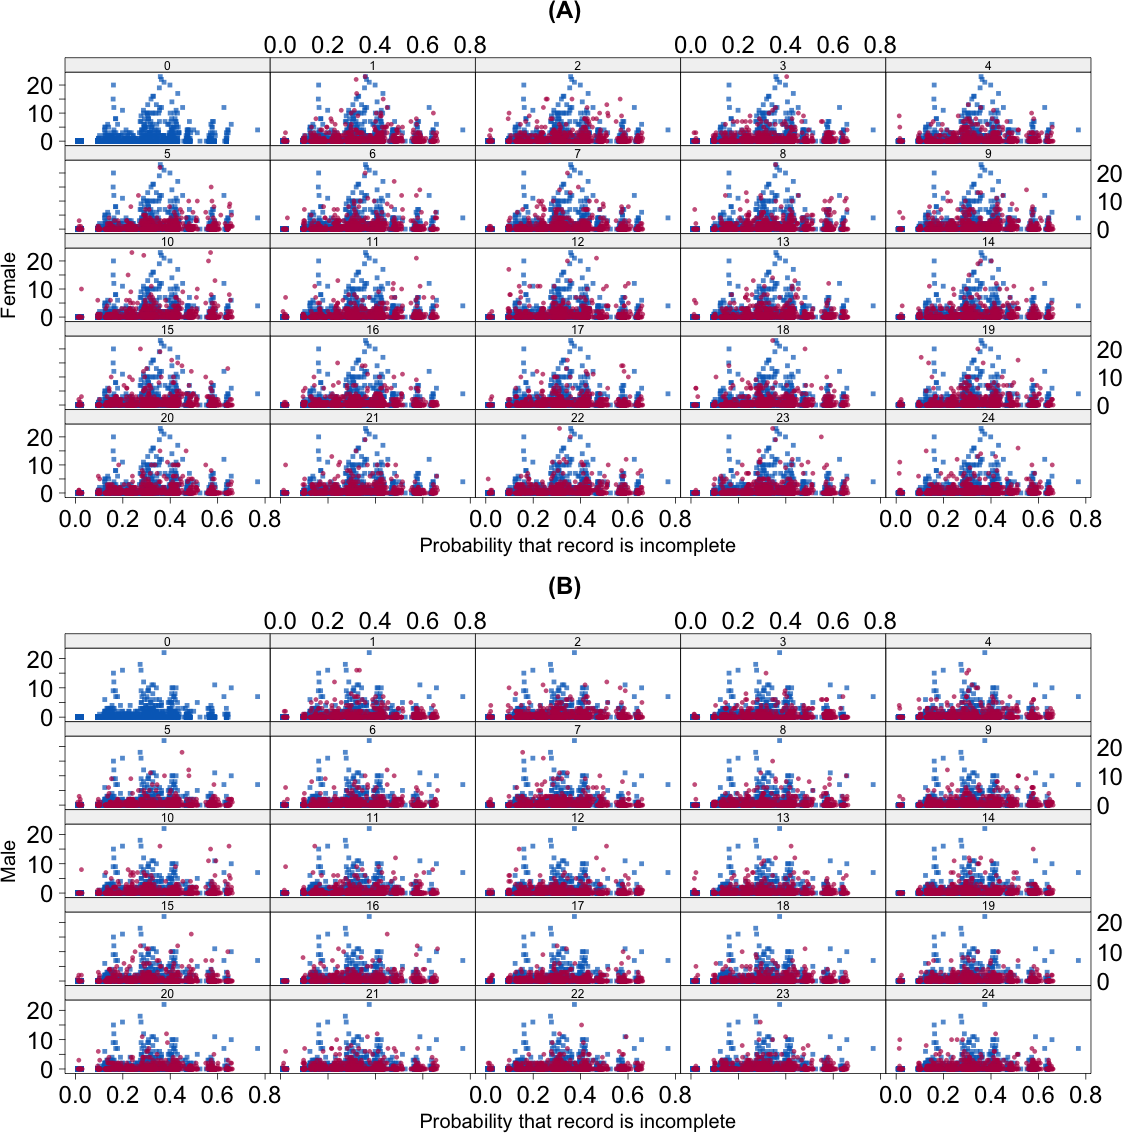
\includegraphics[width=1\linewidth]{kernel-xy-imp1-all-diag-1} \caption{Number of female (A) and male (B) against the missingness probability for observed (data set numbered 0) and imputed data (data set numbered 1 to 24).}\label{fig:kernel-xy-imp1-all-diag}
\end{figure}

\begin{landscape}\begin{table}

\caption{\label{tab:pool-diag}Imputation model indices with different values of m. NAs resulted from nonestimable number of male and female in a treatment. The abbreviations are crop identities, which are the combinations of the first letter in crop species names and the rotation to which the crops belonged.}
\begin{threeparttable}
\centering
\resizebox{\linewidth}{!}{
\begin{tabular}[t]{lrr>{}rrr>{}rrr>{}rrr>{}rrr>{}r}
\toprule
\multicolumn{1}{c}{ } & \multicolumn{3}{c}{n/m} & \multicolumn{3}{c}{riv} & \multicolumn{3}{c}{fmi} & \multicolumn{3}{c}{$\lambda$} & \multicolumn{3}{c}{le} \\
\cmidrule(l{3pt}r{3pt}){2-4} \cmidrule(l{3pt}r{3pt}){5-7} \cmidrule(l{3pt}r{3pt}){8-10} \cmidrule(l{3pt}r{3pt}){11-13} \cmidrule(l{3pt}r{3pt}){14-16}
Term & m = 24 & m = 240 & m = 2400 & m = 24 & m = 240 & m = 2400 & m = 24 & m = 240 & m = 2400 & m = 24 & m = 240 & m = 2400 & m = 24 & m = 240 & m = 2400\\
\midrule
Intercept & 0.2083 & 0.1167 & 0.1433 & 0.3739 & 0.3644 & 0.3386 & 0.2793 & 0.2699 & 0.2554 & 0.2722 & 0.2671 & 0.2529 & 0.0116 & 0.0011 & 0.0001\\
Block: 2 & 0.2083 & 0.1167 & 0.1433 & 0.5344 & 0.5998 & 0.5840 & 0.3575 & 0.3781 & 0.3712 & 0.3483 & 0.3749 & 0.3687 & 0.0149 & 0.0016 & 0.0002\\
Block: 3 & 0.2083 & 0.1167 & 0.1433 & 0.5804 & 0.5371 & 0.5117 & 0.3770 & 0.3525 & 0.3410 & 0.3672 & 0.3494 & 0.3385 & 0.0157 & 0.0015 & 0.0001\\
Block: 4 & 0.2083 & 0.1167 & 0.1433 & 0.9424 & 0.7040 & 0.6527 & 0.4978 & 0.4164 & 0.3975 & 0.4852 & 0.4131 & 0.3949 & 0.0207 & 0.0017 & 0.0002\\
Crop ID: C3 & 0.2083 & 0.1167 & 0.1433 & 0.3516 & 0.4493 & 0.4273 & 0.2669 & 0.3130 & 0.3019 & 0.2601 & 0.3100 & 0.2994 & 0.0111 & 0.0013 & 0.0001\\
Crop ID: C2 & 0.2083 & 0.1167 & 0.1433 & 0.1682 & 0.2340 & 0.2591 & 0.1480 & 0.1923 & 0.2083 & 0.1440 & 0.1896 & 0.2058 & 0.0062 & 0.0008 & 0.0001\\
Crop ID: C4 & 0.2083 & 0.1167 & 0.1433 & 0.8327 & 0.8853 & 0.8554 & 0.4663 & 0.4730 & 0.4636 & 0.4544 & 0.4696 & 0.4610 & 0.0194 & 0.0020 & 0.0002\\
Crop ID: O3 & 0.2083 & 0.1167 & 0.1433 & 0.7229 & 0.6626 & 0.6850 & 0.4307 & 0.4018 & 0.4091 & 0.4196 & 0.3985 & 0.4065 & 0.0179 & 0.0017 & 0.0002\\
Crop ID: A4 & 0.2083 & 0.1167 & 0.1433 & 0.3330 & 0.5269 & 0.5021 & 0.2563 & 0.3482 & 0.3368 & 0.2498 & 0.3451 & 0.3343 & 0.0107 & 0.0015 & 0.0001\\
Crop ID: S2 & 0.2083 & 0.1167 & 0.1433 & 1.5154 & 0.0006 & 0.0009 & 0.6167 & 0.0031 & 0.0034 & 0.6024 & 0.0006 & 0.0009 & 0.0257 & 0.0000 & 0.0000\\
Crop ID: S3 & 0.2083 & 0.1167 & 0.1433 & NA & NA & NA & NA & NA & NA & NA & NA & NA & NA & NA & NA\\
Crop ID: S4 & 0.2083 & 0.1167 & 0.1433 & 0.0006 & NA & NA & 0.0031 & NA & NA & 0.0006 & NA & NA & 0.0001 & NA & NA\\
Corn weed management : low & 0.2083 & 0.1167 & 0.1433 & 0.4410 & 0.4470 & 0.4214 & 0.3140 & 0.3119 & 0.2990 & 0.3060 & 0.3089 & 0.2965 & 0.0131 & 0.0013 & 0.0001\\
Crop ID: C3 x Corn weed management : low & 0.2083 & 0.1167 & 0.1433 & 0.6788 & 0.6881 & 0.6047 & 0.4150 & 0.4109 & 0.3794 & 0.4043 & 0.4076 & 0.3768 & 0.0173 & 0.0017 & 0.0002\\
Crop ID: C2 x Corn weed management : low & 0.2083 & 0.1167 & 0.1433 & 0.4194 & 0.8696 & 0.7311 & 0.3032 & 0.4685 & 0.4249 & 0.2955 & 0.4651 & 0.4223 & 0.0126 & 0.0020 & 0.0002\\
Crop ID: C4 x Corn weed management : low & 0.2083 & 0.1167 & 0.1433 & 1.3038 & 1.0537 & 1.0291 & 0.5798 & 0.5166 & 0.5097 & 0.5659 & 0.5131 & 0.5072 & 0.0242 & 0.0022 & 0.0002\\
Crop ID: O3 x Corn weed management : low & 0.2083 & 0.1167 & 0.1433 & 0.6842 & 0.6712 & 0.8059 & 0.4170 & 0.4049 & 0.4488 & 0.4062 & 0.4016 & 0.4463 & 0.0174 & 0.0017 & 0.0002\\
Crop ID: A4 x Corn weed management : low & 0.2083 & 0.1167 & 0.1433 & 0.2450 & 0.4780 & 0.4938 & 0.2020 & 0.3264 & 0.3331 & 0.1968 & 0.3234 & 0.3306 & 0.0084 & 0.0014 & 0.0001\\
Crop ID: S2 x Corn weed management : low & 0.2083 & 0.1167 & 0.1433 & NA & NA & NA & NA & NA & NA & NA & NA & NA & NA & NA & NA\\
Crop ID: S3 x Corn weed management : low & 0.2083 & 0.1167 & 0.1433 & NA & NA & NA & NA & NA & NA & NA & NA & NA & NA & NA & NA\\
Crop ID: S4 x Corn weed management : low & 0.2083 & 0.1167 & 0.1433 & NA & NA & NA & NA & NA & NA & NA & NA & NA & NA & NA & NA\\
\bottomrule
\end{tabular}}
\begin{tablenotes}[para]
\item \textit{Note:} 
\item{Some zero values are due to rounding.\\  
C2: corn in the 2-year rotation, C3: corn in the 3-year rotation, C4: corn in the 4-year rotation, \\
S2: soybean in the 2-year rotation, S3: soybean in the 3-year rotation, S4: soybean in the 4-year rotation, \\
O3: oat in the 3-year rotation, and A4: alfalfa in the 4-year rotation}
\end{tablenotes}
\end{threeparttable}
\end{table}
\end{landscape}


\begin{landscape}\begin{table}

\caption{\label{tab:sexr19-covar-summ}Numerical diagnosis of model's goodness of fit with and without covariates on 2019 imputed data sets.}
\centering
\resizebox{\linewidth}{!}{
\begin{threeparttable}
\begin{tabular}[t]{l>{}lll>{}llllllllll>{}lllllll>{}l>{}ll>{}l}
\toprule
\addlinespace[0.3em]
\multicolumn{25}{l}{\textbf{(A) Population aboveground mass covariate}}\\
\hspace{1em}Imputation & 1 & 2 & 3 & 4 & \textbf{5} & 6 & \textbf{7} & 8 & 9 & 10 & \textbf{11} & 12 & \textbf{13} & 14 & \textbf{15} & 16 & 17 & 18 & 19 & 20 & 21 & 22 & 23 & \vphantom{2} 24\\
\hspace{1em}Deviance & 45.87 & 42.80 & 34.31 & 36.78 & \textbf{40.89} & 62.70 & \textbf{52.69} & 56.73 & 22.47 & 46.68 & \textbf{39.74} & 38.19 & \textbf{26.05} & 47.66 & \textbf{28.19} & 46.58 & 43.79 & 31.49 & 48.21 & 50.59 & 31.26 & 34.89 & 51.67 & 38.57\\
\hspace{1em}Dispersion & 1.95 & 1.84 & 1.38 & 1.48 & \textbf{1.54} & 2.40 & \textbf{2.14} & 2.38 & 1.05 & 1.93 & \textbf{1.75} & 1.60 & \textbf{1.06} & 2.01 & \textbf{1.22} & 1.90 & 1.61 & 1.24 & 1.87 & 2.19 & 1.37 & 1.36 & 2.09 & 1.50\\
\addlinespace[0.3em]
\multicolumn{25}{l}{\textbf{(B) Population stand density covariate}}\\
\hspace{1em}Imputation & 1 & 2 & 3 & 4 & \textbf{5} & 6 & \textbf{7} & 8 & 9 & 10 & \textbf{11} & 12 & \textbf{13} & 14 & \textbf{15} & 16 & 17 & 18 & 19 & 20 & 21 & 22 & 23 & \vphantom{1} 24\\
\hspace{1em}Deviance & 45.22 & 37.60 & 41.66 & 39.11 & \textbf{52.50} & 66.21 & \textbf{61.79} & 51.69 & 27.44 & 47.33 & \textbf{36.24} & 47.05 & \textbf{28.19} & 44.59 & \textbf{24.53} & 59.57 & 48.72 & 38.23 & 35.92 & 66.81 & 35.47 & 49.25 & 58.26 & 58.51\\
\hspace{1em}Dispersion & 1.98 & 1.62 & 1.67 & 1.58 & \textbf{2.00} & 2.54 & \textbf{2.55} & 2.12 & 1.28 & 1.94 & \textbf{1.59} & 1.99 & \textbf{1.16} & 1.84 & \textbf{1.05} & 2.47 & 1.79 & 1.56 & 1.40 & 2.96 & 1.54 & 1.88 & 2.41 & 2.29\\
\addlinespace[0.3em]
\multicolumn{25}{l}{\textbf{(C) No covariate}}\\
\hspace{1em}Imputation & 1 & 2 & 3 & 4 & \textbf{5} & 6 & \textbf{7} & 8 & 9 & 10 & \textbf{11} & 12 & \textbf{13} & 14 & \textbf{15} & 16 & 17 & 18 & 19 & 20 & 21 & 22 & 23 & 24\\
\hspace{1em}Deviance & 78.24 & 63.29 & 72.17 & 72.88 & \textbf{90.87} & 105.28 & \textbf{91.76} & 81.60 & 49.72 & 73.75 & \textbf{63.36} & 64.03 & \textbf{45.61} & 80.43 & \textbf{47.17} & 95.78 & 75.41 & 57.65 & 72.34 & 96.18 & 68.97 & 69.57 & 96.86 & 87.33\\
\hspace{1em}Dispersion & 2.10 & 1.72 & 1.87 & 1.82 & \textbf{2.12} & 2.56 & \textbf{2.36} & 2.07 & 1.42 & 1.99 & \textbf{1.70} & 1.71 & \textbf{1.19} & 2.03 & \textbf{1.23} & 2.42 & 1.75 & 1.48 & 1.76 & 2.52 & 1.80 & 1.66 & 2.44 & 2.15\\
\bottomrule
\end{tabular}
\begin{tablenotes}[para]
\item \textit{Note: } 
\item Bold columns are imputations that produced full sets of data (six among 24 imputed sets) that allow estimation of the effects of corn weed management on population sex ratio. In these data sets, at least one non-zero value was filled into the Male or Female column that were originally NAs. NA values in the original data set were due to high efficacy of weed control in soybean plots that left no waterhemp plants survived at sex evaluation, which resulted in non-estimable sex ratio.
\end{tablenotes}
\end{threeparttable}}
\end{table}
\end{landscape}
\renewcommand\refname{References}
  \bibliography{fecund.bib}

\end{document}

